\begin{XeClass}{FTPFileSystem}
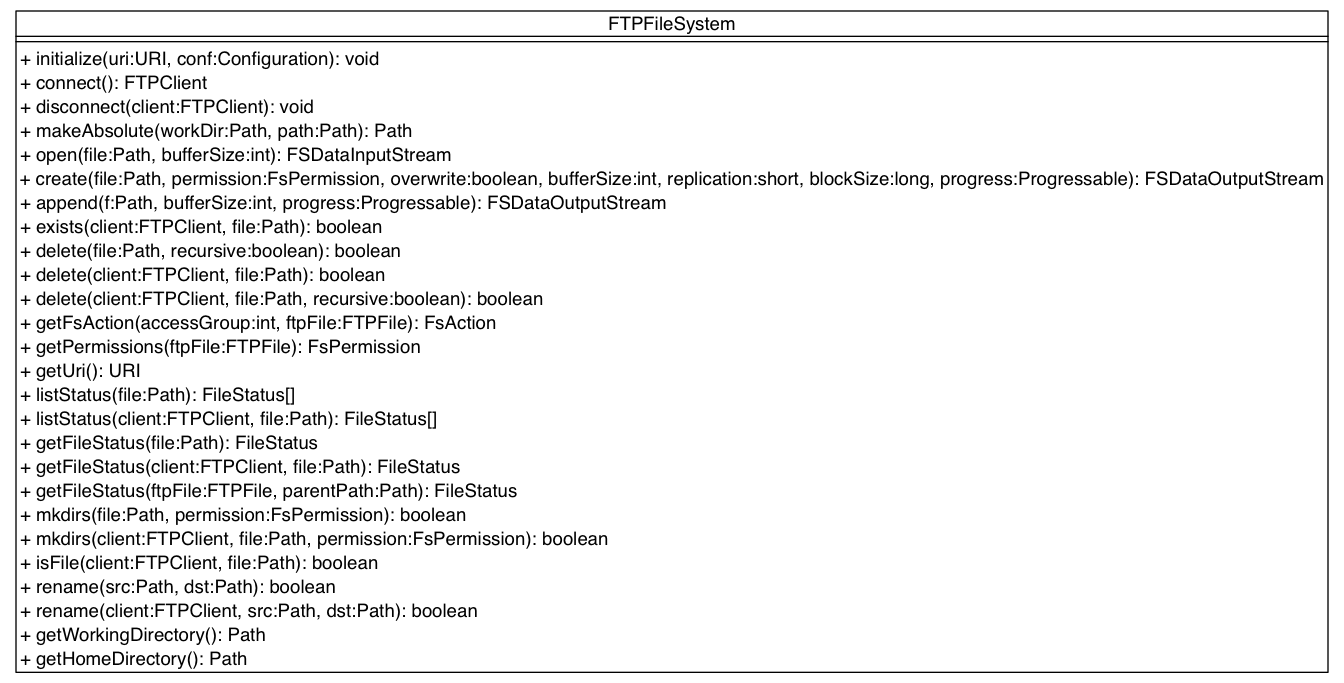
\includegraphics[width=\textwidth]{cdig/FTPFileSystem.png}
     
 由FTP服务器支持的文件系统,基于FTP协议和FTP服务器交互的FileSystem API实现
 继承自\emph{FileSystem}

    \begin{XeMethod}{\XePublic}{void}{initialize}
         
 使用超类FileSystem调用initialize,通过uri获得host,port,和userAndPassword
 初始化的函数通过获得的host,port,user,password配置Configuration对象.
 host通过Configuration对象设置保存在fs.ftp.host
 port通过Configuration对象设置保存在fs.ftp.host.port
 user通过Configuration对象设置保存在"fs.ftp.user." + host
 password通过Configuration对象设置保存在"fs.ftp.password." + host

    \end{XeMethod}

    \begin{XeMethod}{\XePrivate}{FTPClient}{connect}
         
 使用获取得到的Configuration配置FTP Server
 通过在从初始化里保存好的host,port,user,password获取相应的值
 使用FTPClient类生成FTPClient对象,并通过给定主机地址和端口号进行连接
 使用FTPClient对象和从Configuration对象中取出的user和password Sign In
 设置FTP.BLOCK_TRANSFER_MODE,FTP.BINARY_FILE_TYPE and DEFAULT_BUFFER_SIZE

    \end{XeMethod}

    \begin{XeMethod}{\XePrivate}{void}{disconnect}
         
 FTPFileSystem类断开连接API
 判断FTPClient对象是否为null,不为null则进一步判断是否没有连接
 当判断为有连接,则通过FTPClient调用disconnect方法断开连接
 logoutSuccess记录断开连接登出的状态,判断是否断开连接成功

    \end{XeMethod}

    \begin{XeMethod}{\XePrivate}{Path}{makeAbsolute}
         
 通过给定workDir工作目录和path路径

    \end{XeMethod}

    \begin{XeMethod}{\XePublic}{FSDataInputStream}{open}
         
 open函数接收两个参数,Path对象file和基本数据类型int bufferSize
 获得连接的FTPClient对象,并得到工作目录的绝对路径
 判断fileStat是不是一个目录,若是则断开FTPClient对象client连接
 通过client获得bufferSize大小的字节数
 获得当前工作目录的父路径,只有这样才能在使用InputStream状态下读
 当在FSDataInputStream内调用close()方法,FTPClient对象断开连接
 当FTPClient对象处于inconsistent状态,则要在FTP Server端登出和断开连接,并关闭文件流操作

    \end{XeMethod}

    \begin{XeMethod}{\XePublic}{FSDataOutputStream}{create}
         
 create方法获得连接的FTPClient对象,并得到工作目录的绝对路径
 判断client对象是否存在file路径并判断是否被重写了,若存在,并重写了则删了这个路径,不然则断开FTPClient连接
 抛出异常IOException("File already exists: " + file)
 获得当前工作目录的父路径,若没有父路径或者无法在父路径中有可写准许,则断开FTPClient连接
 通过client获得bufferSize大小的字节数
 当在FSDataInputStream内FTPClient对象调用close()方法,FTPClient对象断开连接
 当FTPClient对象处于inconsistent状态,则要在FTP Server端登出和断开连接,并关闭文件流操作

    \end{XeMethod}

    \begin{XeMethod}{\XePublic}{FSDataOutputStream}{append}
         
 append方法目前尚不支持 

    \end{XeMethod}

    \begin{XeMethod}{\XePrivate}{boolean}{exists}
         
 exists方法可以不需要打开一个新的连接可以判断FTPClient对象client是否有文件目录file

    \end{XeMethod}

    \begin{XeMethod}{\XePublic}{boolean}{delete}
         
 Override的delete方法通过传入文件目录file,当recursive为true,使用建立连接的FTPClient对象删除这个文件目录

    \end{XeMethod}

    \begin{XeMethod}{\XePrivate}{boolean}{delete}
         
 delete装饰器调用delete(Path file, boolean recursive)方法

    \end{XeMethod}

    \begin{XeMethod}{\XePrivate}{boolean}{delete}
         
 获得client的工作目录并与file组合得到文件目录的绝对路径
 获得绝对路径下的所有文件,并调用delete方法全部删除

    \end{XeMethod}

    \begin{XeMethod}{\XePrivate}{FsAction}{getFsAction}
         
 判断ftpFile与accessGroup是否有可读允许,有则将FsAction对象action赋值为FsAction.READ
 判断ftpFile与accessGroup是否有可写允许,有则将FsAction对象action赋值为FsAction.WRITE
 判断ftpFile与accessGroup是否有可操作允许,有则将FsAction对象action赋值为FsAction.EXECUTE

    \end{XeMethod}

    \begin{XeMethod}{\XePrivate}{FsPermission}{getPermissions}
         
 通过给user,group,others设置FsAction属性,创建FsPermission对象并返回

    \end{XeMethod}

    \begin{XeMethod}{\XePublic}{URI}{getUri}
         
 返回uri格式

    \end{XeMethod}

    \begin{XeMethod}{\XePublic}{FileStatus[]}{listStatus}
         
 使用FTPClient对象client获得连接,并返回当前文件目录下的文件列表

    \end{XeMethod}

    \begin{XeMethod}{\XePrivate}{FileStatus[]}{listStatus}
         
 listStatus方法也是与上述方法实现类似功能,获得当前FTPClient对象client的工作目录
 然后获取其绝对路径,最后返回绝对路径下的所有文件列表.

    \end{XeMethod}

    \begin{XeMethod}{\XePublic}{FileStatus}{getFileStatus}
         
 通过getFileStatus的参数file,获得FTPClient对象client文件目录的状态

    \end{XeMethod}

    \begin{XeMethod}{\XePrivate}{FileStatus}{getFileStatus}
         
 获取当前工作路径的绝对路径,再获得绝对路径的父路径
 若父路径不存在,则对它进行设置
 若父路径存在,则遍历其文件列表,判断是否存在ftpFile.getName()  file.getName()
 若存在则继续递归下去寻找getFileStatus(ftpFile, parentPath)

    \end{XeMethod}

    \begin{XeMethod}{\XePrivate}{FileStatus}{getFileStatus}
         
 覆盖在FTPFile\emph{FileStatus}文件目录信息
 使用默认的blockSize当FTP Client不清楚Server的Block Size

    \end{XeMethod}

    \begin{XeMethod}{\XePublic}{boolean}{mkdirs}
         
 使用FTPClient对象client获得连接,并判断是否能创建文件目录

    \end{XeMethod}

    \begin{XeMethod}{\XePrivate}{boolean}{mkdirs}
         
 通过给定的client,file和permission判断是否可以在当前工作目录的绝对路径下创建一个文件目录

    \end{XeMethod}

    \begin{XeMethod}{\XePrivate}{boolean}{isFile}
         
 通过调用getFileStatus(client, file).isFile()方法判断当前client实例在file目录下是否存在文件目录

    \end{XeMethod}

    \begin{XeMethod}{\XePublic}{boolean}{rename}
         
 调用 rename(FTPClient client, Path src, Path dst)函数,并返回结果

    \end{XeMethod}

    \begin{XeMethod}{\XePrivate}{boolean}{rename}
         
 获取src的绝对路径和dst的绝对路径,若src的绝对路径的父路径与dst的不相等,则无法重命名
 重命名成功后则返回true

    \end{XeMethod}

    \begin{XeMethod}{\XePublic}{Path}{getWorkingDirectory}
         
 调用getHomeDirectory()返回home文件路径

    \end{XeMethod}

    \begin{XeMethod}{\XePublic}{Path}{getHomeDirectory}
         
 返回当前工作目录Path

    \end{XeMethod}

\end{XeClass}
